\section{MODELO LIVIANO DE NEGOCIO}

El objetivo de este capítulo es presentar el modelo de negocio de la solución desde una perspectiva de la innovación. En primera instancia se presenta lo que actualmente existe en el mercado asociado a los \textit{meetingware} en segundo lugar se identifica el marco de trabajo - desarrollado con la metodología \textit{Startup Lean} - donde se sitúa el producto a desarrollar. Pasando por el segmento de usuarios al cual está dirigido; luego, se presenta la propuesta de valor además de los canales del producto para ir finalizando con las ventajas competitivas del producto D-Minute.

\subsection{\textit{MEETINGWARE} COMERCIALES}

Antes de generar nuestro marco de trabajo es importante analizar las herramientas del mercado que poseen funcionalidades para el seguimiento de reuniones puesto que muchos productos de mercado abordan los temas que hemos analizado en capítulos anteriores. Lo anterior nos permite conocer a la competencia para establecer nuestra oferta de valor y ventaja competitiva.

A continuación se listan \textit{software} del mercado de más importancia\footnote{Los software de mercado fueron seleccionados desde \url{https://comparisons.financesonline.com/projectplace-software-vs-workep}}


\begin{enumerate}[1.]
    \item \textbf{Projectplace\footnote{\url{https://www.projectplace.com/}}}
    \begin{enumerate}[a]
	    \item \underline{Descripción:} Es una herramienta que permite a las empresas lograr sus objetivos por medio de la gestión de proyectos conjunta, facilitando la comunicación y colaboración del equipo. 
		\item \underline{Características:} Posee herramientas de planificación de proyectos, administración de tareas, gestión de documentos y gestión de reuniones. Permite realizar reuniones en línea, gestionar la cartera de proyectos y sus recursos, generar informes y notificaciones para realizar actividades de control. Es reconocido por sus excelentes medidas de seguridad. Comunicación en tiempo real a través de la fuente de conversación que fomenta la colaboración. Es compatible con aplicaciones móviles iOS y Android. Posee APIs que permite integración con otros \textit{software}.
	    \item \underline{Beneficios:} Facilita la colaboración al conocer las actividades principales, los hitos, las prioridades y proyectos del equipo independiente de donde se ubique cada miembro. Permite hacer seguimiento en línea de las tareas del equipo identificando alertas a tiempo cuando hay desvíos del foco. Permite que cada miembro tenga el control de su trabajo y los compromisos personales. Ofrece un punto de encuentro donde los empleados organizan reuniones en línea, comparten opiniones y archivos, teniendo todos acceso a la información necesaria. Una ventaja distintiva es que permite compartir archivos directamente desde sus cuentas de Google, Box o Dropbox. Posee el mecanismo de inicio de sesión único (Single Sign-On, SSO) que entrega un marco de identificación eficaz para evitar la pérdida de datos. En resumen es una única plataforma que centraliza todas las actividades relacionadas con la gestión de proyectos.
	    \item \underline{Precio:}  Existe sólo un plan a \$29.00 por usuario al mes, aunque para aquellos que deseen conocerla existe una versión de prueba gratis. La versión pagada incluye todas las características ya mencionadas. 
    \end{enumerate}	
    \item \textbf{Attentiv\footnote{\url{http://attentiv.com/}}}
    \begin{enumerate}[a]
	    \item \underline{Descripción:} Es una plataforma en la nube que busca mejorar la colaboración de los equipos y la toma de decisiones por medio de chat, votaciones, encuestas y comentarios. Es una herramienta que puede reducir los tiempos de reunión y ayudar a mejorar la cultura de la empresa. 
		\item \underline{Características:} Permite iniciar conversaciones en equipo, sea de forma anónima o no. También permite a los usuarios votar por los comentarios de los demás y filtrar los comentarios basados en estos votos ascendentes. Los usuarios pueden crear encuestas personalizadas para la respuesta del equipo y pueden organizar debates en diferentes grupos. 
	    \item \underline{Beneficios:} Con esta plataforma se puede obtener retroalimentación anónima o no y en línea. Permite destacar las buenas ideas que nacen de los equipos por medio de las votaciones. Este software fomenta tener menos reuniones, más efectivas y llegar a decisiones mejores y más informadas.
	    \item \underline{Precio:} Posee versión gratuita para grupos pequeños. Los grupos más grandes requieren una suscripción mensual. Versión gratis: hasta 10 usuarios, 1 GB de almacenamiento, encuestas y discusiones ilimitadas. Si requiere más capacidad tiene un costo de USD\$ 5 por usuario mensual, e incluye usuarios Ilimitados, almacenamiento de 20 GB, encuestas y discusiones ilimitadas. Por último, si aún se requiere mayor capacidad existe la versión a USD\$ 7 por usuarios mensual, que considera usuarios Ilimitados, almacenamiento de 20 GB, encuestas y discusiones ilimitadas.
    \end{enumerate}	    
    \item \textbf{Agreedo\footnote{\url{https://www.agreedo.com/es/index.html}}}
    \begin{enumerate}[a]
	    \item \underline{Descripción:} Es una aplicación orientada a la administración de reuniones. Su objetivo es capturar toda aquella información relevante que surge en cada reunión como lo son tareas, compromisos y decisiones. Permite compartir notas personales a otros miembros. 
		\item \underline{Características:} Programar reuniones y crear minutas, integración con distintos correos electrónicos (Outlook, Google Calendar, Lotus Notes, etc.). Seguridad del contenido basado en encriptación SSL. 
	    \item \underline{Beneficios:} Permite crear minutas estructuradas de reuniones, las cuales puedes compartir fácilmente. Permite hacer seguimiento de los compromisos de la reunión anterior, para aumentar la efectividad de éstas.
	    \item \underline{Precio:} La estructura de precios está compuesta por 3 versiones; gratis, premium y enterprise. La primera permite programar reuniones, crear minutas, sumar participantes y archivos de forma limitada. Integrarse con algún correo electrónico, además de poseer encriptación de contenido. La segunda tiene un costo de US\$ 7/mes (usuario único) o US\$ 60/mes (10 usuarios), y cuenta con las mismas funciones que la versión básica pero reuniones, participantes y archivos adjuntos ilimitados. Por último, existe la versión dirigida a empresas, la cual incluye las mismas características de la versión Premium más 100 MB de límite de tamaño de archivo adjunto.
    \end{enumerate}	    
    \item \textbf{Kairos\footnote{\url{https://kairos.lat/}}}
    \begin{enumerate}[a]
	    \item \underline{Descripción:} Es una plataforma orientada a eficientar el tiempo empleado en reuniones teniendo un propósito claro para lograr mayor productividad. Facilita el cumplimiento de tareas y entrega claridad sobre lo que se debe lograr por medio de su sistema de seguimiento y reportes.  
		\item \underline{Características:} Cuenta con agenda y dashboard donde se visualizan las próximas reuniones y tareas pendientes. Se pueden crear minutas rápidas y fáciles capturando acuerdos y compromisos con fecha de resolución, y además puedes asignarles responsables. Puedes enviar minutas por correo electrónico. Permite registrar avances de las tareas para realizar seguimiento. Está integrado con Google calendar para crear reuniones dentro y fuera de la plataforma, con Google Drive para adjuntar archivos y que todos manejen la misma información, y con Asana para dar seguimiento al cumplimiento de las tareas acordadas en tus reuniones.
	    \item \underline{Beneficios:} Esta plataforma tiene la capacidad de integrarse con las principales herramientas de administración de tareas; Asana, Google o Slack. Registra minutas, acuerdos y compromisos evitando malos entendidos. Posee herramientas de agenda y organización efectiva. Entrega reportería dirigida a la alta dirección sobre el desempeño del equipo. Organiza, registra y da seguimiento a acuerdos y tareas. Entrega visión clara sobre lo que se tiene que lograr y las tareas a realizar para cada integrante y a nivel global. 
	    \item \underline{Precio:} Existe la alternativa gratis que posee límite de hasta 3 usuarios. Por USD\$8 al mes permite interactuar hasta 25 usuarios, y en plan anual por USD\$7.
    \end{enumerate}	    
    \item \textbf{Evernote\footnote{\url{https://evernote.com/intl/es}}}    
    \begin{enumerate}[a]
	    \item \underline{Descripción:} Es una herramienta que permite capturar y compartir notas en cualquier formato (video, imagen, archivo de audio o notas escritas a mano), facilitando su búsqueda en cualquier dispositivo o lugar.
		\item \underline{Características:} Permite generar, editar y marcar texto, realizar bocetos y formas rápidamente. Cuenta con interfaz móvil y web. Permite almacenar notas, clips web, archivos e imágenes. Cuenta con geolocalización. Facilita la colaboración y creación compartiendo tus ideas con otras personas.  
	    \item \underline{Beneficios:} Permite almacenar distintos elementos dentro de una nota. Permite organizar reuniones rápidas y efectivas utilizando las notas almacenadas las cuales pueden transformarse fácilmente en presentaciones amigables.
	    \item \underline{Precio:} Existen 4 planes opcionales. El básico es sin costo e incluye poder compartir notas con acceso a 2 dispositivos. El Plus tiene un costo de US\$ 3.99/ mes o US\$ 34.99/año. Este tiene una capacidad mensual de 1GB en nuevas cargas, se sincroniza con todos tus dispositivos, permite buscar texto dentro de las imágenes, puedes compartir notas con otras personas, incluye soporte y puedes acceder sin conexión. El Premium tiene un  costo de USD\$ 7.99/mes o US\$ 69.99/año. Permite 10 GB de nuevas cargas por mes, todas las funciones del Plus más buscar texto y editar PDF. La versión para empresas tiene un costo por usuario al mes de US\$ 14.99, incluye 20 GB de nuevas cargas al mes más 2 GB por usuario. Adicional a las características de la versión Premium cuenta con inicio de sesión único y administración central de usuarios.
    \end{enumerate}	    
    \item \textbf{Workep\footnote{\url{https://workep.com/es/es.html}}}    
    \begin{enumerate}[a]
	    \item \underline{Descripción:} Es una plataforma para la gestión de proyectos que permite a los equipos trabajar de forma conjunta sin importar la locación de sus miembros, desarrollada especialmente para trabajar con la Suite Google.  
		\item \underline{Características:} Administración de tareas, búsqueda general de proyectos, tareas y contactos, manejo de gantt, integración con aplicaciones de Google, notificaciones de correo electrónico inteligente.
	    \item \underline{Beneficios:} Ayuda a que los equipos de proyecto permanezcan coordinados durante la vida del proyecto. Posee gráficas detalladas que dan claridad sobre los proyectos y su progreso. Organiza y centraliza toda los archivos y otros materiales de contenido. Al ser una plataforma que de forma nativa está diseñada para integrarse a las herramientas Google, facilita su adopción por la familiaridad de éstas para las personas y empresas. Facilita la comunicación y trabajo en equipo en todo lugar y momento con sus herramientas; Calendar, Drive, Hangouts, entre otras. 
	    \item \underline{Precio:} Existe la versión gratis que incluye la plataforma básica; tareas, proyectos y archivos ilimitados, hasta 10 miembros del equipo, solo 1 equipo, integraciones con G Suite. Otra opción es la versión escalable, con un costo mensual de \$2.99 por usuario. Esta incluye las mismas características de la versión gratis, pero no restringe el número de equipos ni miembros. Además ofrece roles y soporte prioritario. Finalmente existe la opción Crecimiento la cual contiene las mismas características de la versión antes mencionada, sin embargo adiciona plantillas de proyecto, dependencias de tareas, gantt avanzado, Rastreador de tiempo, búsqueda universal y marca personalizada. Su costo es de \$4.99/usuario por mes.
    \end{enumerate}	      
\end{enumerate}

\subsection{MARCO DE LA INNOVACIÓN}

Para generar el marco de la innovación del software D-Minute se utilizó la metodología \textit{Lean Startup} desarrollada por Eric Ries \fullcite{RN29}, el cual es una guía para: establecer el segmento de clientes que tendrá foco el proyecto, sus oportunidades respecto al mercado, los flujos de ingreso que podría alcanzar la plataforma para el retorno de la inversión y su propuesta de valor diferenciada. Estos puntos son relevantes para establecer los canales de difusión, la estructura de costos necesaria para iniciar el desarrollo y la ventaja competitiva respecto al mercado. Lo anterior nos va permitir generar el lienzo del modelo de negocio para D-Minute.

\subsubsection{Segmento de destinatarios}

La mayoría de empresas hoy en día requieren de reuniones de trabajo para el seguimiento de tareas, por tanto el segmento importante que requiera de un sistema de minutas es: proveedores de \textit{software} a medida, servicios de consultoría, bancos, servicios públicos, empresas de obra gruesa y ONGs.

\subsubsection{Oportunidades}

Como hemos detectado en CAPÍTULO 1, CAPÍTULO 2 y en base a lo que hemos recogido de los \textit{meetingware} comerciales. Se observan funcionalidades que deben estar presente en programas que coordinan equipos de trabajo, hacen seguimiento a tareas y compromisos, definen alcances y funcionalidades, comprometen recursos entre otras actividades. Dichas oportunidades son:

\begin{enumerate}[1.]
	\item Debe incorporar el concepto de “proyecto” como el conjunto de reuniones
	\item Recorrer las reuniones anteriores con flexibilidad y pertinencia. 
	\item Aplicar elementos que sinteticen la convergencia y la divergencia de argumentos de manera explícita
	\item Permitir editar los elementos del hilo argumental de la reunión y que son fruto de las discusiones al interior del equipo de desarrollo. En el caso de la teoría de diálogo/acción son los acuerdos, desacuerdos, dudas y compromisos.
	\item Registrar tareas que nacen de los compromisos individuales de forma automática y de una manera visual para seguimiento.
\end{enumerate}

\subsubsection{Flujos de ingreso}

Toda solución requiere conocer la forma que se recupera la inversión, dado los costos que existen por herramientas de este tipo se detecta que los flujos de ingreso se pueden dar por: 

\begin{enumerate}[1.]
	\item Modelo de suscripción
	\item Arriendo del servicio por reunión - Flat Rate 
	\item Publicidad en costados - Uso financiado por publicidad
	\item Arriendo de la plataforma - \textit{White Label}
\end{enumerate}

Lo anterior considerando que el producto pasa por generación, adopción y mejora continua como ciclo de vida de costo.

\subsubsection{Propuesta de valor}

Generar reuniones efectivas es el gran desafío que se presenta en el área del \textit{meetingware} debido a los costos directos e indirectos que se generan por esta instancia. La propuesta de valor se enfoca en criterios que devuelvan la efectividad a las reuniones en los equipos creativos y agilizando las reuniones de proyecto con una síntesis del diálogo.

Los criterios son los siguientes:

\begin{enumerate}[1.]
	\item \textbf{Usable}, en otras palabras se espera que todas sus componentes para manejar sets de reuniones de un proyecto exhiba usabilidad.
	\item \textbf{Trazable}, es decir, el sistema debe tener una forma visual de administrar las relaciones causales entre los elementos dialógicos que se dan en las reuniones: acuerdos, compromisos, dudas y desacuerdos.
	\item \textbf{Buscable}; quiere decir que siempre habrá filtros para encontrar lo que se busca de las reuniones.
	\item \textbf{Accionable}, que por medio de un tablero Kanban de reuniones se generen tareas para un elemento del dialógico, el compromiso individual.
\end{enumerate}


\subsubsection{Canales}

Se identifica que el medio por el que se hará llegar la propuesta de valor al segmento de clientes, se da por regalar el producto en una ONGs para “envirar” el ambiente empresarial, cuentas oficiales de D-Minute (Instagram, youtube, twitter y facebook), conversación con oficina de proyecto (PMO) empresariales y oferta del producto por web diferenciada por tamaño de empresa.

\subsubsection{Recursos claves}

Con el fin de garantizar una implementación correcta del producto es necesario conocer qué tipo de recursos son claves para el éxito, en este caso hemos detectado:

\begin{enumerate}[1.]
	\item Servicio cloud con escalamiento dinámico
	\item Desarrollador \textit{fullstack} en el uso de micro arquitectura
	\item Notebook de desarrollo
	\item Servidor de Dominio 
\end{enumerate}

\subsubsection{Estructura de costos}

Para operar el modelo de negocio se debe incurrir en costos que permitan operar, por tanto la estructura debe considerar: costos de creación y entrega de valor, relaciones con cliente y generación de ingresos. 

Las siguientes preguntas definen la estructura de costos:

\begin{enumerate}[1.]
	\item ¿Cuáles son los costos más importantes para mantener el modelo de negocio? 
	
	\textbf{R:} Diseño UX, Servidor de dominio, Programador \textit{fullstack} y \textit{Cloud Service}.
	\item ¿Cuáles son los recursos claves más caros? 
	
	\textbf{R:} \textit{Cloud Service} y Programador \textit{fullstack}
	\item ¿Cuáles son las actividades claves más caras? 

	\textbf{R:} Programación 

	\item ¿Qué actividades claves están realizando nuestros socios? 
	
	\textbf{R:} Programación
\end{enumerate}

\subsubsection{Ventaja competitiva como emprendimiento}

Esta parte se pone como frases de marketing y en este caso son las siguientes: 

\begin{enumerate}[1.]
	\item Conocemos de \textit{meetingware}, management y comunicación efectiva.
	\item Nuestro trabajo se basa en un paper sobre la teoría del diálogo y en una tesis de Magíster que prueba la efectividad del método dialógico.
	\item Soporte de \textit{couching} de comunicación efectiva en empresas
\end{enumerate}

\subsubsection{Lienzo D-Minute}

El lienzo Canvas es el resumen de nuestro temas abordados y representa nuestro modelo de negocio para nuestro mínimo producto viable (en adelante MVP, del inglés \textit{Minimum Viable Product}), representado en imagen \ref{img3-1}.

\begin{figure}[h]
\centering
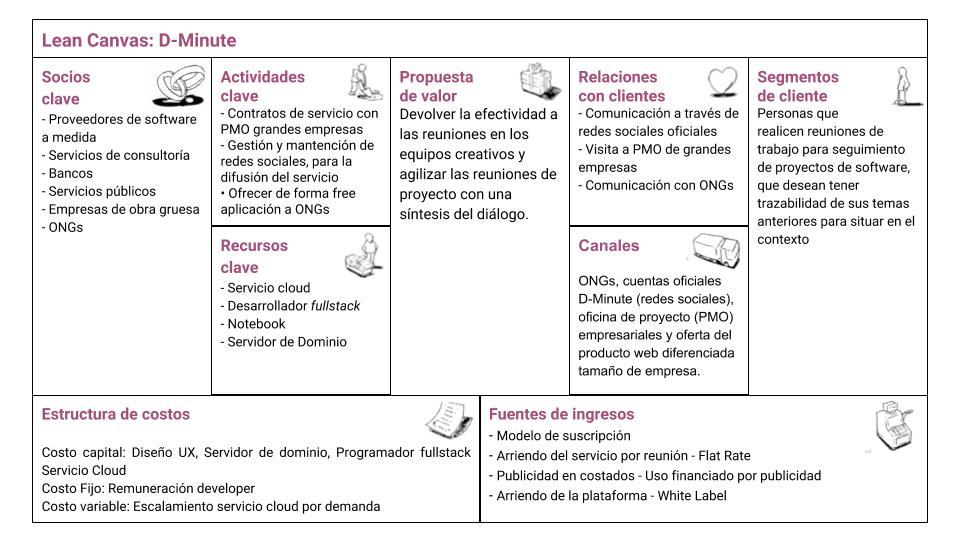
\includegraphics[width=1\linewidth]{/LeanCanvas}
\caption{Lienzo Canvas D-Minute, tomado de Lean Canvas y elaboración propia} 
\label{img3-1}
\end{figure}

\subsection{\textit{BENCHMARKING}}

El \textit{benchmarking}\footnote{Benchmarking para más información acerca de esto ver los siguiente enlaces \url{https://www.economiasimple.net/glosario/benchmarking} y \url{https://es.wikipedia.org/wiki/Benchmarking} } aplicado a D-Minute corresponde a la categoría funcional pues nos hemos orientado a competidores directos como indirectos - un ejemplo de competidor indirecto es Evernote dado que no es un software de reuniones pero es de uso frecuente en ellas - con la finalidad de responder los criterios de evaluación de cada productos. Cada criterio está basado en la literatura expuesta en el marco conceptual del CAPÍTULO 2, el cual menciona que es lo mínimo que debe poseer un sistema de reuniones para ser un apoyo y no al revés, ver imagen \ref{img3-2}.

\begin{figure}[h]
\centering
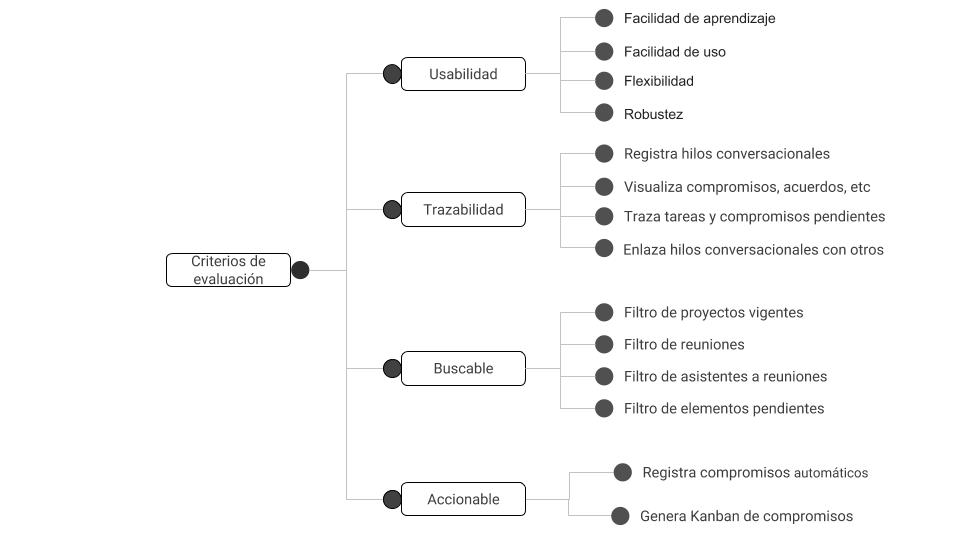
\includegraphics[width=1\linewidth]{/CriteriosBenchmark}
\caption{Criterios evaluados para un \textit{meetingware}, elaboración propia} 
\label{img3-2}
\end{figure}

Se ha definido cuatro pilares de evaluación de nivel macro pues son la base para un gestor de reuniones y por cada pilar se establecen subcriterios de evaluación que nos permiten identificar si los sistemas poseen al menos una de las funcionalidades del pilar. Por último, para determinar cuan efectiva es una herramienta se asigna un porcentaje de relevancia a cada uno de los pilares y sub-pilares, estos valores fueron obtenidos de encuestas realizadas a gestores de proyecto que a diario se ven enfrentados a reuniones de trabajo, ver anexo A.  Los datos estan representadas en las tablas \ref{tab:usable} - \ref{tab:trazable} - \ref{tab:buscable} - \ref{tab:accionable} que contienen: Item\footnote{Corresponde a la descripción evaluada del criterio}, Porcentaje Nota Obtenida\footnote{Nota Obtenida: corresponde a la suma de los promedios obtenidos por la cantidad de personas encuestadas}, Q. Respuesta\footnote{Q de Respuesta: corresponde al número de personas que respondió el sub criterio.}.

\begin{table}[!h]
\centering
\caption{Resultado criterio Usable, elaboración propia}
\label{tab:usable}
\begin{tabular}{|l|r|r|}
\hline
\multicolumn{3}{|c|}{Criterio Usable} \\ \hline
\multicolumn{1}{|c|}{Ítem} & \multicolumn{1}{c|}{Porcentaje Nota Obtenida} & \multicolumn{1}{c|}{Q. Respuesta} \\ \hline
Facilidad de aprendizaje & 33.3 & 7 \\ \hline
Facilidad de uso & 85,7 & 18 \\ \hline
Flexibilidad & 47,6 & 10 \\ \hline
Robustez & 52,4 & 11 \\ \hline
\end{tabular}
\end{table}

\begin{table}[!h]
\centering
\caption{Resultado criterio Trazable, elaboración propia}
\label{tab:trazable}
\begin{tabular}{|l|r|r|}
\hline
\multicolumn{3}{|c|}{Criterio Trazable} \\ \hline
\multicolumn{1}{|c|}{Ítem} & \multicolumn{1}{c|}{Porcentaje Nota Obtenida} & \multicolumn{1}{c|}{Q. Respuesta} \\ \hline
Registra hilos conversacionales & 81 & 17 \\ \hline
Traza tareas y compromisos pendientes & 66,7 & 14 \\ \hline
Enlaza hilos conversacionales con otros & 38,1 & 8 \\ \hline
\end{tabular}
\end{table}

\begin{table}[!h]
\centering
\caption{Resultado criterio Buscable, elaboración propia}
\label{tab:buscable}
\begin{tabular}{|l|r|r|}
\hline
\multicolumn{3}{|c|}{Criterio Buscable} \\ \hline
\multicolumn{1}{|c|}{Ítem} & \multicolumn{1}{c|}{Porcentaje Nota Obtenida} & \multicolumn{1}{c|}{Q. Respuesta} \\ \hline
Filtro de proyectos vigentes & 71,4 & 15 \\ \hline
Filtro de reuniones & 85,7 & 18 \\ \hline
Filtro de asistentes a reuniones & 47,6 & 10 \\ \hline
Filtro de elementos pendientes & 71,4 & 15 \\ \hline
\end{tabular}
\end{table}

\begin{table}[!h]
\centering
\caption{Resultado criterio Accionable, elaboración propia}
\label{tab:accionable}
\begin{tabular}{|l|r|r|}
\hline
\multicolumn{3}{|c|}{Criterio Accionable} \\ \hline
\multicolumn{1}{|c|}{Ítem} & \multicolumn{1}{c|}{Porcentaje Nota Obtenida} & \multicolumn{1}{c|}{Q. Respuesta} \\ \hline
Registra compromisos automáticos & 52,4 & 11 \\ \hline
Genera Kanban de compromisos & 81 & 17 \\ \hline
\end{tabular}
\end{table}

\begin{table}[!h]
\centering
\caption{Resultado encuesta de criterios, elaboración propia}
\label{tab:resultado}
\begin{tabular}{|l|r|r|}
\hline
\multicolumn{1}{|c|}{Criterio} & \multicolumn{1}{c|}{Nota Promedio} & \multicolumn{1}{c|}{Nota final} \\ \hline
Usable & 81 & 17 \\ \hline
Trazable & 81 & 17 \\ \hline
Buscable & 52,4 & 11 \\ \hline
Accionable & 81 & 17 \\ \hline
\end{tabular}
\end{table}

De los datos capturados se calculó el promedio de la nota obtenida por criterio con el fin de establecer cuál de ellos posee una mayor relevancia para los encuestados y a su vez determinar el porcentaje final de cada criterio en escala de 1 a 100, en términos porcentuales, ver imagen \ref{img3-3}.


\begin{figure}[!h]
\centering
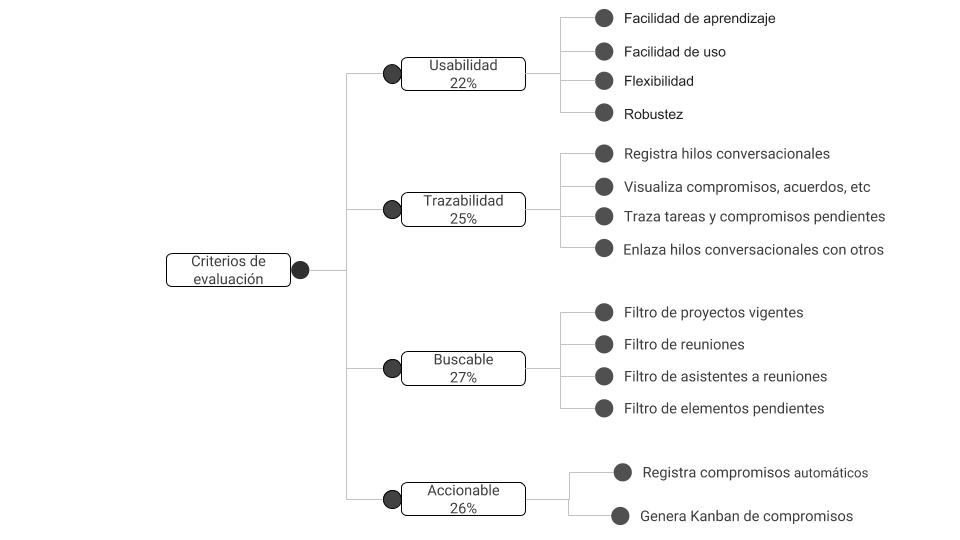
\includegraphics[width=1\linewidth]{/CriteriosBenchmarkPorcentaje}
\caption{Resultado criterio de evaluación \textit{meetingware}, elaboración propia} 
\label{img3-3}
\end{figure}

Para determinar la nota final de cada criterio con la Ecuación 1, se utilizó el promedio de cada uno - ver tabla \ref{tab:resultado} - sobre la suma de los promedios, determinando de esta forma la importancia relativa en términos porcentuales.

Si bien los datos muestran que todos los sistemas poseen a lo menos tres de cuatro pilares. El pilar de trazabilidad es uno de los más relevantes en el contexto de reuniones el cual coindice con lo expone por: \fullcite{RN24}, \fullcite{RN15}, \fullcite{RN37}, \fullcite{RN16} entre otros mencionados en el CAPÍTULO 2 sección 2.3, debido a que trabajar con una síntesis dialógica mejora y sitúa en contexto a los participantes de una reunión. D-Minute posee los cuatro pilares pues y uno de los focos es la síntesis del diálogo expuesta por \fullcite{RN24}, donde se centra este software y trabajo, ver resultado en tabla \ref{tab:resultadoevaluacion}.

\begin{table}[!h]
\centering
\caption{Resultado evaluación de \textit{meetingware}, elaboración propia}
\label{tab:resultadoevaluacion}
\resizebox{15cm}{!} {
\begin{tabular}{|l|l|c|c|c|c|c|c|c|}
\hline
\multicolumn{1}{|c|}{Pilar} & \multicolumn{1}{c|}{Criterio} & D-Minute & Projectplace & Attentiv & Agreedo & Kairos & Evernote & Workep \\ \hline
\multicolumn{1}{|c|}{\multirow{4}{*}{Usabilidad}} & Facilidad de aprendizaje & x &  & x &  & x & x & x \\ \cline{2-9} 
\multicolumn{1}{|c|}{} & Facilidad de uso & x &  & x & x & x & x & x \\ \cline{2-9} 
\multicolumn{1}{|c|}{} & Flexibilidad & x & x &  &  &  & x & x \\ \cline{2-9} 
\multicolumn{1}{|c|}{} & Robustez & x & x &  &  & x & x & x \\ \hline
\multirow{4}{*}{Trazabilidad} & Registra elementos de diálogo & x & x &  & x & x &  &  \\ \cline{2-9} 
 & Visualiza elementos de diálogo & x & x &  & x & x &  &  \\ \cline{2-9} 
 & Traza elementos de diálogo pendientes & x & x &  &  & x &  &  \\ \cline{2-9} 
 & Enlaza elementos de diálogo & x &  &  &  &  &  &  \\ \hline
\multirow{4}{*}{Buscable} & Filtro de proyectos vigentes & x & x &  &  &  & x & x \\ \cline{2-9} 
 & Filtro de reuniones & x &  &  & x &  & x & x \\ \cline{2-9} 
 & Filtro de asistentes a reuniones & x &  &  &  &  & x &  \\ \cline{2-9} 
 & Filtro de elementos pendientes & x &  &  &  &  &  &  \\ \hline
\multirow{2}{*}{Accionable} & Registra compromisos automáticos & x &  &  &  &  &  & x \\ \cline{2-9} 
 & Genera Kanban de compromisos &  &  &  &  & x &  &  \\ \hline
\end{tabular}
}
\end{table}

En consecuencia, con los criterios de comparación establecidos y en igualdad de condiciones tenemos una clara ventaja de D-Minute en relación a todas las herramienta que se analizaron en esta tesis. 88\% es un número lo suficientemente significativo para demostrar la ventaja de la herramienta que se propone en este tesis de magister, el resultado se puede ver en la tabla \ref{tab:evaluacionfinal}.

\begin{table}[!h]
\centering
\caption{Cálculo del peso de los \textit{meetingware} evaluados, elaboración propia}
\label{tab:evaluacionfinal}
\resizebox{15cm}{!} {
\begin{tabular}{cl|r|r|r|r|r|r|r|}
\cline{3-9}
\multicolumn{1}{l}{} &  & \multicolumn{7}{c|}{\textbf{Meetingware}} \\ \cline{3-9} 
\multicolumn{1}{l}{} & \multicolumn{1}{c|}{} & \multicolumn{1}{c|}{D-Minute} & \multicolumn{1}{c|}{Projectplace} & \multicolumn{1}{c|}{Attentiv} & \multicolumn{1}{c|}{Agreedo} & \multicolumn{1}{c|}{Kairos} & \multicolumn{1}{c|}{Evernote} & \multicolumn{1}{c|}{Workep} \\ \hline
\multicolumn{1}{|c|}{\multirow{4}{*}{\textbf{Porcentaje Pilar}}} & Usabilidad (22\%) & 22 & 11 & 11 & 5,5 & 16,5 & 22 & 22 \\ \cline{2-9} 
\multicolumn{1}{|c|}{} & Trazabilidad (25\%) & 24 & 18 & 0 & 12 & 18 & 0 & 0 \\ \cline{2-9} 
\multicolumn{1}{|c|}{} & Buscable (27\%) & 28 & 7 & 0 & 7 & 0 & 21 & 14 \\ \cline{2-9} 
\multicolumn{1}{|c|}{} & Accionable (26) & 13,5 & 0 & 0 & 0 & 0 & 0 & 13,5 \\ \hline
\multicolumn{2}{|r|}{\textbf{Totales}} & \textbf{88\%} & \textbf{36\%} & \textbf{11\%} & \textbf{25\%} & \textbf{35\%} & \textbf{43\%} & \textbf{50\%} \\ \hline
\end{tabular}

}
\end{table}


\subsection{RESUMEN}

El presente capítulo expone los diferentes software de mercado que permiten hacer seguimiento a reuniones de proyecto. Por cada \textit{software} se analizaron las características sus beneficios, los factores relevantes de cada herramienta y por último su valor de mercado. Esto nos genera una fuente valiosa de información que se hace relevante a la hora conocer si nuestro MVP es un producto viable, usable y competitivo. 

Dado el análisis anterior, en la segunda parte del capítulo fue generado el marco de innovación del \textit{software} D-Minute representado en el lienzo “Lean Canvas” de la aplicación D-Minute.

Para concluir se realizó un \textit{benchmarking} de los diferentes sistemas revisados y se aplicó un cuadro comparativo de los criterios de evaluación analizados en el capítulo uno y dos, para determinar cómo se sitúa D-Minute en el mercado.

En los próximos capítulos se va presentar el desarrollo de la solución y en forma posterior establecer los criterios de evaluación que nos permitan validar las preguntas de investigación más allá del mercado.

